\documentclass{standalone}
\usepackage{tikz}
\begin{document}
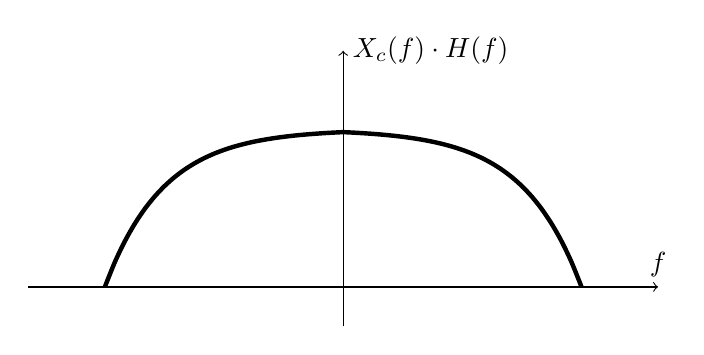
\begin{tikzpicture}[scale=2]
    \draw[->](-2,0)--(2,0)node[above]{$f$};
    \draw[->](0,-0.25)--(0,1.5)node[right]{$X_c(f)\cdot H(f)$};

    \draw[ultra thick]plot[smooth, domain=0:1.513](\x,{1-0.25*e^(2.7*(\x-1))});
    \draw[ultra thick]plot[smooth, domain=-1.513:0](\x,{1-0.25*e^(-2.7*(\x+1))});
\end{tikzpicture}
\end{document}